\documentclass[10pt,xcolor=table]{beamer}
\usetheme{Warsaw}
\usecolortheme{dolphin}
\usepackage[utf8]{inputenc}
\usepackage[spanish]{babel}
\usepackage{amsmath}
\usepackage{amsfonts}
\usepackage{amssymb}
\usepackage{graphicx}
\usepackage{multimedia}
\usepackage{booktabs}
\author[Cindy Castell\'on]{{\footnotesize Presentado por}\\
	Cindy Mariella Castellón Salguero\\
	\vspace{0.2 cm}
	{\footnotesize Asesorado por}\\
	Ph. D. Hermes Le\'on Vargas \\
	M. Sc. Ra\'ul Antonio Henr\'iquez Ort\'iz }
	
\title[Estudio de la componente mu\'onica de cascadas atmosf\'ericas]{{\normalsize Proyecto de trabajo de graduaci\'on:} \\ \vspace{0.5 cm}
\textbf{\textit{Estudio de la componente mu\'onica en la distribuci\'on lateral de cascadas atmosf\'ericas}}}
%\setbeamercovered{transparent} 
\setbeamertemplate{headline}{}
\setbeamertemplate{navigation symbols}{} 
\setbeamertemplate{footline}{}
% set the footline
\setbeamertemplate{footline}{
  \hbox{%
% left block with the shortname, it is set in the \author command
    \begin{beamercolorbox}[wd=.30\paperwidth,ht=2.25ex,dp=1ex,center]%
      {author in head/foot}%
      \usebeamerfont{author in head/foot}\insertshortauthor
    \end{beamercolorbox}%
% center block with the short title, it is set in the \title command
    \begin{beamercolorbox}[wd=.60\paperwidth,ht=2.25ex,dp=1ex,center]%
      {title in head/foot}%
      \usebeamerfont{title in head/foot}\insertshorttitle
    \end{beamercolorbox}%
% right block with the number of slides
    \begin{beamercolorbox}[wd=.10\paperwidth,ht=2.25ex,dp=1ex,right]%
      {date in head/foot}%
      \usebeamerfont{date in head/foot}
      \insertframenumber{} / \inserttotalframenumber\hspace*{1em}
    \end{beamercolorbox}}%
  \vskip0pt%
}

\makeatletter
\setbeamertemplate{frametitle}{%
  \nointerlineskip%
  \vskip-2pt%
  \hbox{\leavevmode
    \advance\beamer@leftmargin by -12bp%
    \advance\beamer@rightmargin by -12bp%
    \beamer@tempdim=\textwidth%
    \advance\beamer@tempdim by \beamer@leftmargin%
    \advance\beamer@tempdim by \beamer@rightmargin%
    \hskip-\Gm@lmargin\hbox{%
      \setbox\beamer@tempbox=\hbox{\begin{minipage}[b]{\paperwidth}%
          \vbox{}\vskip-.75ex%
          \vspace{0.14cm}% <- change here to whatever you want
          \leftskip0.3cm%
          \rightskip0.3cm plus1fil\leavevmode
          \usebeamercolor[fg]{frametitle}\usebeamerfont{frametitle}\strut\insertframetitle\strut\par%
          \ifx\insertframesubtitle\@empty\else%
            {\usebeamerfont*{framesubtitle}{\usebeamercolor[fg]{framesubtitle}\insertframesubtitle}\strut\par}%
          \fi%
          \nointerlineskip
          \vspace{0.1cm}
          \vbox{}%
          \end{minipage}}%
      \beamer@tempdim=\ht\beamer@tempbox%
      \advance\beamer@tempdim by 2pt%
      \begin{pgfpicture}{0pt}{0pt}{\paperwidth}{\beamer@tempdim}
        \usebeamercolor{frametitle right}
        \pgfpathrectangle{\pgfpointorigin}{\pgfpoint{\paperwidth}{\beamer@tempdim}}
        \pgfusepath{clip}
        \pgftext[left,base]{\pgfuseshading{beamer@frametitleshade}}
      \end{pgfpicture}
      \hskip-\paperwidth%
      \box\beamer@tempbox%
    }%
    \hskip-\Gm@rmargin%
  }%
  \nointerlineskip
    \vskip-0.2pt
    \hbox to\textwidth{\hskip-\Gm@lmargin\pgfuseshading{beamer@topshade}\hskip-\Gm@rmargin}
    \vskip-2pt
}

\mode<presentation> {
% coloring for slides other options: beetle, dove
  \usecolortheme{dolphin}
% to include a slide with the table of contents
 \AtBeginSection[] {
  \begin{frame}
    \tableofcontents[currentsection]
  \end{frame} }
}

%\logo{} 
\institute{Escuela de Física, Facultad de Ciencias Naturales y Matem\'atica \\ Universidad de El Salvador} 
\date{} 
\subject{Proyecto de investigación} 



\begin{document}

\begin{frame}
\titlepage
\end{frame}

\begin{frame}
\tableofcontents
\end{frame}

\section{Marco Teórico}
\begin{frame}{Rayos cósmicos}
	\begin{columns}
		\begin{column}{0.35\textwidth}
		Descubiertos por Victor Hess en 1912; los rayos c\'osmicos son partículas cargadas originadas en ambientes extremos del universo, que llegan a la Tierra con altas energías ($>10^9$ eV).
%			\begin{block}{ }
%			Descubiertos por Victor Hess en 1912; los rayos c\'osmicos son partículas cargadas originadas en ambientes extremos del universo, que llegan a la Tierra con altas energías ($>10^9$ eV).
%			\end{block}
			\vspace{\fill}
		\end{column}
		\begin{column}{0.65\textwidth}
			\begin{figure}
			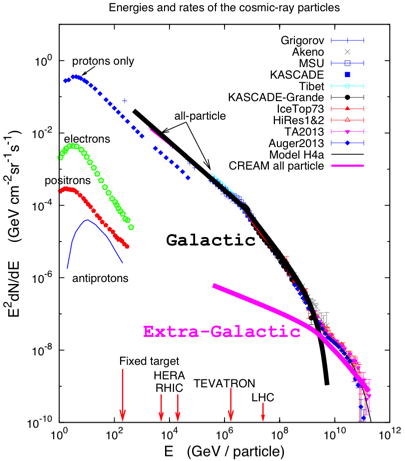
\includegraphics[width=0.9\textwidth, height=0.75\textheight]{Figuras/cr-energy} 
			\caption{Espectro de rayos c\'osmicos (Gaisser, 2013).}
			\end{figure}				
		\end{column}			
	\end{columns}	
\end{frame}

\begin{frame}
\begin{columns}
		\begin{column}{0.5\textwidth}
		\center
		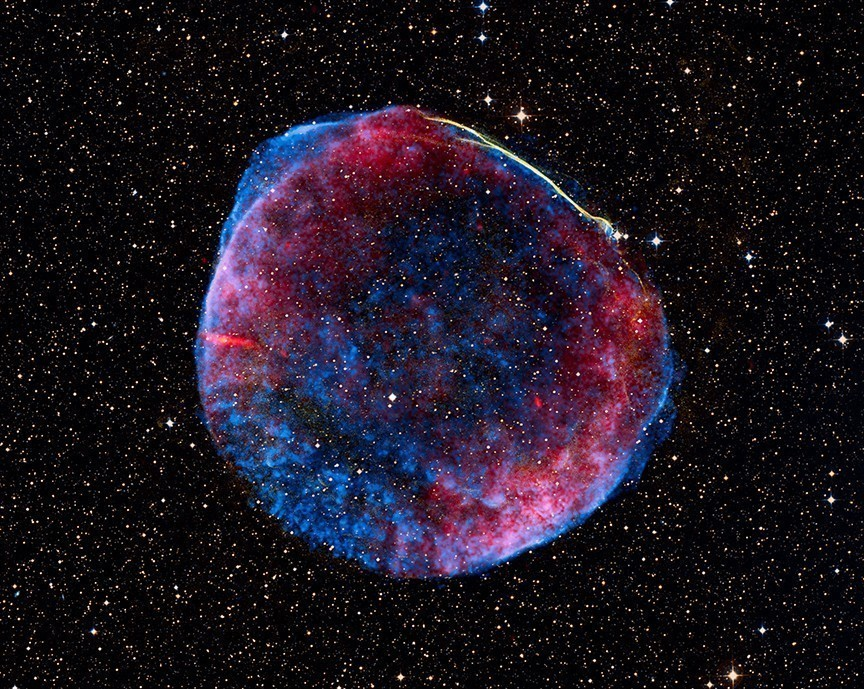
\includegraphics[width=1\textwidth]{Figuras/snr}
		\end{column}
		
		\begin{column}{0.5\textwidth}
		\center
		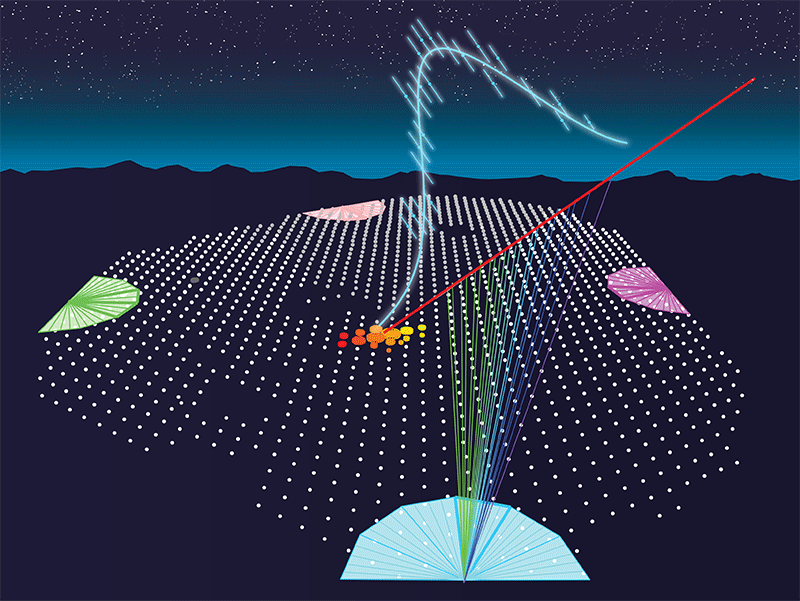
\includegraphics[width=1\textwidth]{Figuras/surfacedetector}
		\end{column}
\end{columns}
\end{frame}

\begin{frame}{Cascadas Atmosf\'ericas}
	\begin{figure}
	\centering
	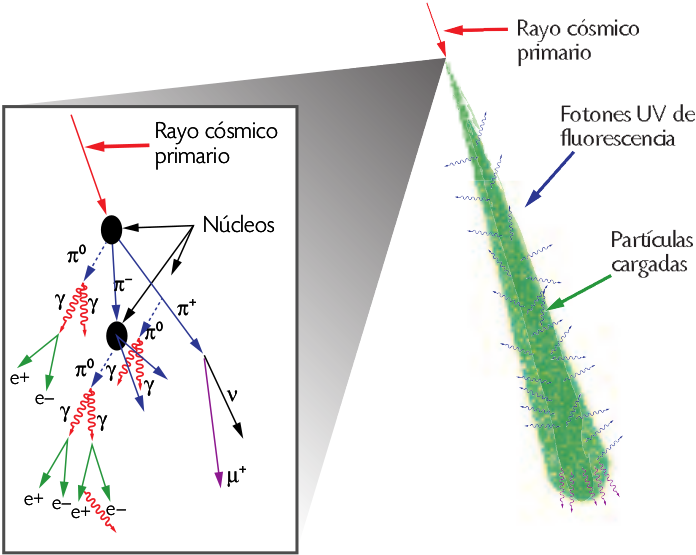
\includegraphics[width=0.75\textwidth]{Figuras/air_shower} 
	\caption{Esquema de formación y desarrollo de una cascada (Bahena, 2013).}
	\label{fig:airshower}
	\end{figure}	
\end{frame}	

\begin{frame}{Muones en cascadas}
Los muones se producen principalmente en decaimiento de mesones: \vspace{0.5 cm}
	\begin{LARGE}
	\textcolor{blue} {
		\begin{align*}
		\pi^{\pm}	&\longrightarrow 	\mu^{\pm} + \nu_{\mu}(\bar{\nu}_{\mu})
		\end{align*}
		\begin{align*}
		K^{\pm}		&\longrightarrow 	\mu^{\pm} + \nu_{\mu}(\bar{\nu}_{\mu})
		\end{align*}
	}
	\end{LARGE}

%ideas: -muones vienen de decaimiento de mesones
%- numero de muones depende de E0 y de A
%-muones viven lo suficiente para ser detectados en el suelo
%- muones tienen cross section peque;a asi que no interactuan antes de llegar al suelo.
\end{frame}
	
%\begin{frame}{Detecci\'on de muones}
%deteccion a nivel del suelo y deteccion subterranea.
%
%no se si esto es necesario mejor no ponerlo y podr[ian ser dos diapositivas de HAWC una con la foto y otra con grafiquitas de papers.
%\end{frame}

\begin{frame}{HAWC}
\textit{The High-Altitude Water Cherenkov gamma-ray observatory} (HAWC), a 4100 m s. n. m detecta part\'iculas producidas en cascadas atmosf\'ericas de energ\'ias entre 1 y 100 TeV. \vspace{0.3cm}
	\begin{columns}
		\begin{column}{0.7\textwidth}
		\center
		\href{run:Figuras/HAWC.mov?autostart&loop&start=2&stop=120}
       {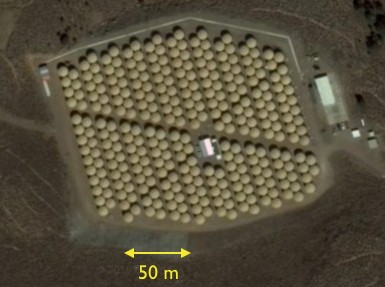
\includegraphics[width=1\textwidth]{Figuras/hawc-array}}
%		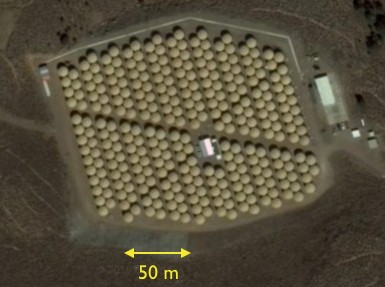
\includegraphics[width=1\textwidth]{Figuras/hawc-array}
		\end{column}
		
		\begin{column}{0.3\textwidth}
		\center
		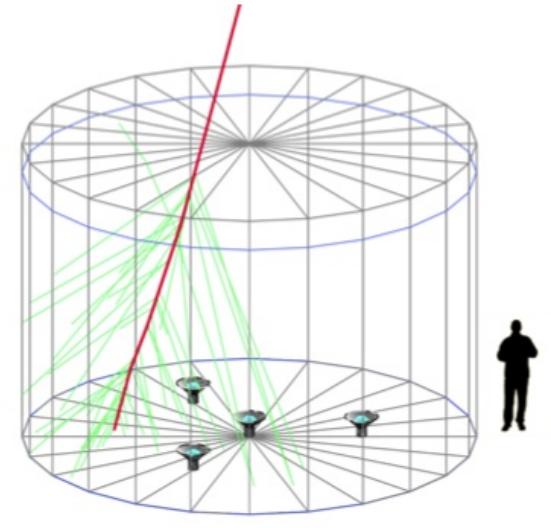
\includegraphics[width=0.9\textwidth]{Figuras/hawc-tank}
		(Figuras de la colaboraci\'on HAWC)
		\end{column}
	\end{columns}

%ideas - foto de hawc
%- rango de energias 1-100 TeV
%-detectan particulas por radiacion de cherenkov en el agua.
%- que se ha hecho con hawc: anisotropia, antiprotones y fuentes galacticas de RC.
\end{frame}
	
%	\begin{frame}{Modelos de chubascos}
%		\begin{block}{Sección eficaz}
%		Probabilidad de que una partícula interactúe.
%		\end{block}	
%		\vspace{5 mm}
%		\begin{block}{Multiplicidad}
%		Número de mesones producidos en una interacción hadrónica.
%		\end{block}	
%		\vspace{5 mm}
%		\begin{block}{Inelasticidad}
%		Fracción de la energía que se invierte en producción de mesones.
%		\end{block}			
%	\end{frame}		
	
	

\section{Planteamiento del problema}

\begin{frame}{Preguntas de investigación}
	\begin{itemize}
	\item ?`Cu\'ales son las caracter\'isticas de la componente mu\'onica de la distribuci\'on lateral de part\'iculas producidas en cascadas? \vspace{0.3 cm}
	\item ?`C\'omo depende dicha componente mu\'onica de la energ\'ia y la masa de la part\'icula primaria? \vspace{0.3 cm}
	\item ?`Son estas dependencias sensibles al modelo de interacciones hadr\'onicas?
	\end{itemize}
\end{frame}

\begin{frame}{Objetivos}
	\begin{block}{Objetivo general}
	Estudiar mediante simulaciones computacionales la distribución lateral de muones en cascadas atmosféricas con energías iniciales en el rango del observatorio HAWC (1-100 TeV).
	\end{block}
	\vspace{0.3 cm}
	\begin{block}{Objetivos espec\'ificos}
		\begin{enumerate}
		\item Caracterizar la densidad de muones a varias distancias del eje de la cascada atmosf\'erica en funci\'on de la energ\'ia inicial. \vspace{0.1 cm}
		\item Comparar las distribuciones de muones en cascadas atmosf\'ericas iniciadas por distintas part\'iculas primarias. \vspace{0.1 cm}
		\item Evaluar la influencia del modelo de interacciones hadr\'onicas de altas energ\'ias utilizado en las simulaciones sobre la distribuci\'on lateral de muones. \vspace{0.1 cm}
		\end{enumerate}
	\end{block}
\end{frame}

\begin{frame}{Justificaci\'on}
\vspace{\fill}
	\begin{itemize}
	\item La distribuci\'on lateral de muones puede usarse en observatorios como HAWC para determinar aspectos como la energ\'ia y la masa del rayo c\'osmico primario. \vspace{0.3 cm}
	\item La caracterizaci\'on de la componente mu\'onica es importante para distinguir cascadas iniciadas por rayos gamma de las iniciadas por rayos c\'osmicos.\vspace{0.3 cm}
	\item El comportamiento de la densidad de muones en simulaciones contrastado con su medici\'on experimental ayuda a mejorar los modelos de interacciones hadr\'onicas. 
	\end{itemize}
\vspace{\fill}
\end{frame}

\begin{frame}{Viabilidad}
\vspace{\fill}
	\begin{itemize}
	\item El sistema AIRES es de acceso libre y está disponible en línea en el sitio \url{http://aires.fisica.unlp.edu.ar/} junto con toda su documentaci\'on. \vspace{0.5 cm}
	\item Se han realizado ejecuciones de prueba en una computadora personal, con lo que se estima un m\'aximo de nueve semanas para realizar las simulaciones. \vspace{0.5 cm}
	\item Para el an\'alisis de datos se utilizar\'an tambi\'en herramientas de acceso libre.
	\end{itemize}
\vspace{\fill}
\end{frame}

\section{Metodología}

\begin{frame}{Sistema AIRES}
\vspace{\fill}
	\begin{center}
	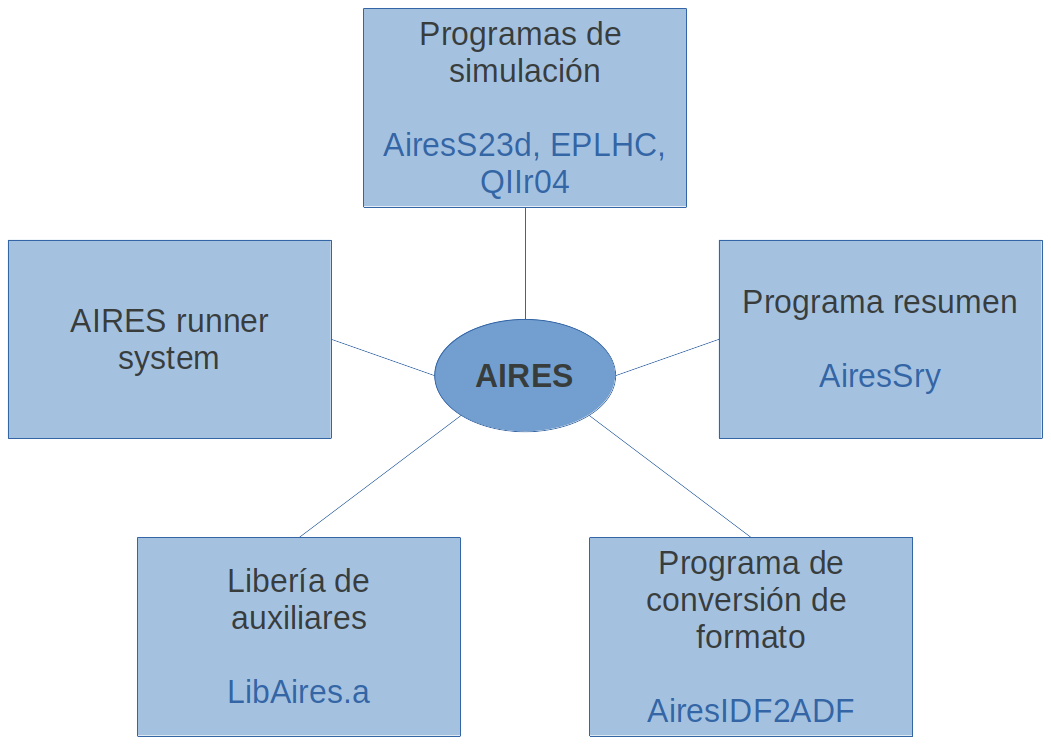
\includegraphics[height=0.8\textheight]{Figuras/airesprograms}
	\end{center}
\vspace{\fill}
\end{frame}

\begin{frame}{Interacciones}
\vspace{\fill}
En AIRES se toman en cuenta los procesos m\'as relevantes para los rayos c\'osmicos en la atm\'osfera: \vspace{0.5 cm}
	\begin{columns}
		\begin{column}{0.5\textwidth}
			\begin{block}{Electrodin\'amicos}
				\begin{itemize}
				\item Producci\'on de pares.
				\item \textit{Bremsstrahlung}.
				\item Efecto fotoel\'ectrico.
				\item Efecto Compton.
				\end{itemize}
			\end{block}
		\end{column}
		\begin{column}{0.5\textwidth}
			\begin{block}{Hadr\'onicos}
			\vspace{0.225 cm}
				\begin{itemize}
				\item Colisiones hadr\'on - n\'ucleo.
				\item Reacciones fotonucleares.
				\item Fragmentaci\'on nuclear.
				\end{itemize}
			\vspace{0.255 cm}
			\end{block}
		\end{column}
	\end{columns}
	\vspace{0.5 cm}
	Adem\'as de decaimientos y procesos de propagaci\'on como ionizaci\'on del medio y dispersi\'on de Coulomb.
	\vspace{\fill}
\end{frame}

\begin{frame}{Programas de simulaci\'on}
\vspace{\fill}
	\begin{center}
	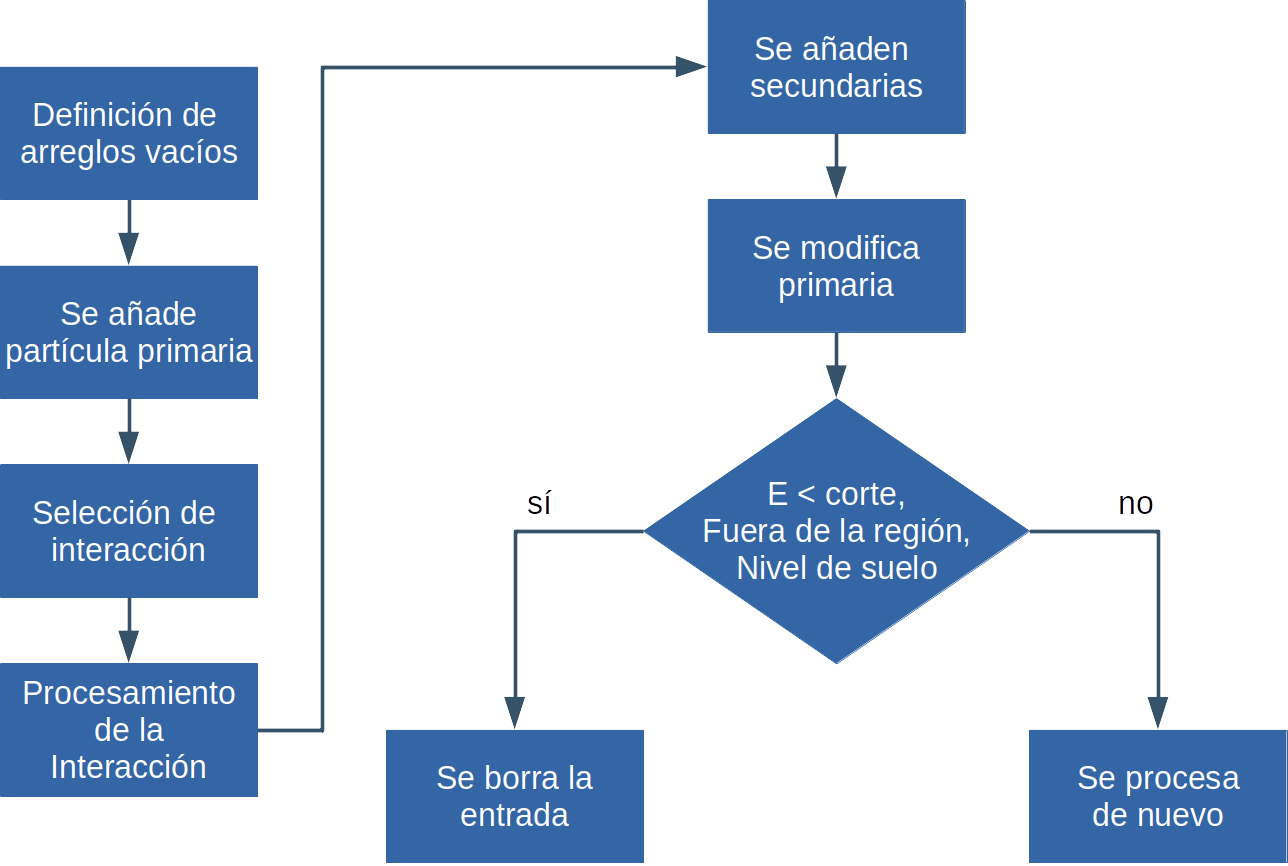
\includegraphics[width=1\textwidth]{Figuras/programdiagram}
	\end{center}
\vspace{\fill}
\end{frame}

\begin{frame}{Simulaciones de cascadas}
	\begin{columns}
		\begin{column}{0.6\textwidth}
		Con cada uno de los tres modelos de interacciones hadrónicas de altas energías (Sibyll 2.3d, EPOS-LHC y QGSJETII-04) se simular\'an aproximadamente 20,000 eventos. \\ \vspace{0.5 cm}
		La ubicaci\'on ser\'a la del observatorio HAWC en Puebla, M\'exico, con latitud de 19$^{o}$ y altura de 4100 m sobre el nivel del mar.
		\end{column}
		
		\begin{column}{0.4\textwidth}
		\begin{block}
		
			\begin{table}[]
				\begin{tabular}{@{}cl@{}}
				{\color[HTML]{0E3EF0} Part\'icula} & p, Fe           \\ \midrule
				{\color[HTML]{0E3EF0} $E_0$}       & $1-100$ TeV     \\ \midrule
				{\color[HTML]{0E3EF0} $\theta_0$}  & $0-45^{\circ}$  \\ \midrule
				{\color[HTML]{0E3EF0} $\phi_0$}    & $0-360^{\circ}$
				\end{tabular}
			\end{table}
		\end{block}
		\end{column}
	\end{columns}
\end{frame}

\section{Cronograma de actividades}

\begin{frame}{Cronograma de actividades}
	\begin{table}[]
		\begin{tabular}{@{}ll@{}}
		\toprule
		\multicolumn{1}{c}{\textbf{Actividad}}                      & \multicolumn{1}{c}{\textbf{Fechas}} \\ \midrule
		\multicolumn{1}{l}{Revisi\'on de bibliograf\'ia}           & 26/09 - 17/12/21 (12 semanas)    \\ \midrule
		\multicolumn{1}{l}{Creaci\'on de archivos de entrada}      & 26/09 - 01/10/21 (1 semana)      \\ \midrule
		\multicolumn{1}{l}{Simulaciones con Sibyll 2.3d}           & 04/10 - 23/10/21 (3 semanas)     \\ \midrule
		\multicolumn{1}{l}{Simulaciones con EPOS-LHC}              & 24/10 - 12/11/21 (3 semanas)     \\ \midrule
		\multicolumn{1}{l}{Simulaciones con QGSJETII-04}           & 13/11 - 04/12/21 (3 semanas)     \\ \midrule
		\multicolumn{1}{l}{Tratamiento y an\'alisis de resultados} & 25/10 - 17/12/21 (6 semanas)     \\ \midrule
		\multicolumn{1}{l}{Comparaci\'on entre los modelos}        & 03/01 - 22/01/22 (3 semanas)     \\ \midrule
		\multicolumn{1}{l}{Redacci\'on del documento final}        & 03/01 - 25/02/22 (8 semanas)     \\ \bottomrule
		\end{tabular}
	\end{table}
\end{frame}

%--------------------------
% Resultados preliminares
%--------------------------
\begin{frame}[noframenumbering]
	\begin{Huge}
	Ap\'endice: \\
	
	resultados preliminares
	\end{Huge}
\end{frame}

\begin{frame}[noframenumbering]
\center
	\begin{figure}
	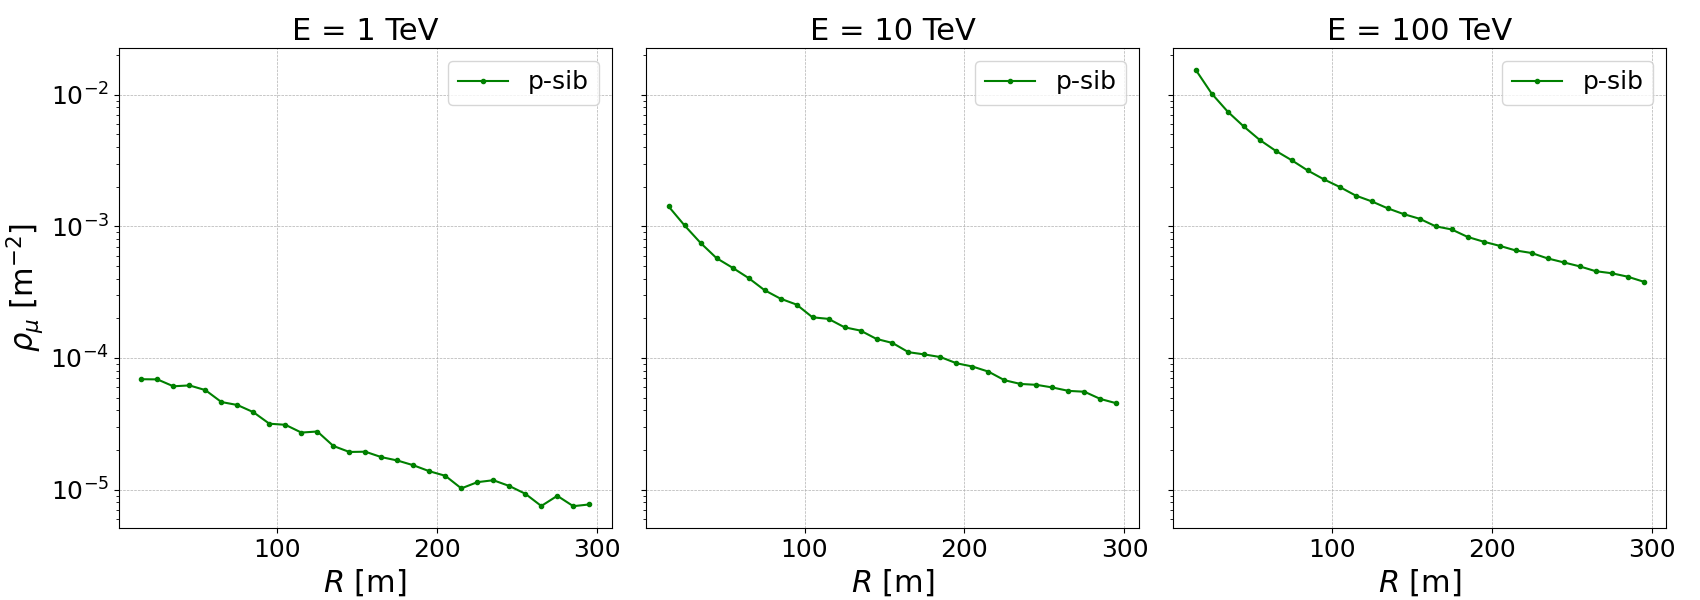
\includegraphics[height=0.4\textheight]{Figuras/lateraldist-psib}
	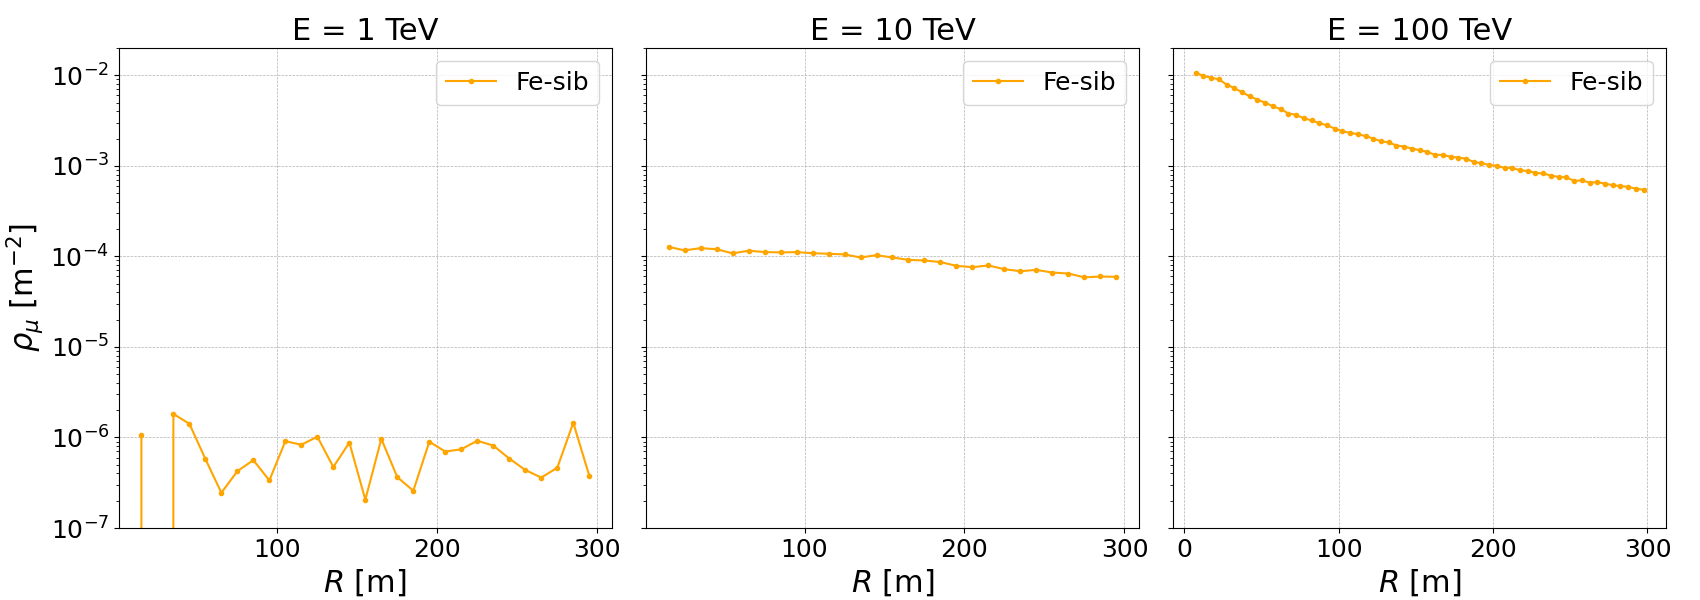
\includegraphics[height=0.4\textheight]{Figuras/lateraldist-Fesib}
	\caption{Resultados preliminares de distribuci\'on lateral de muones con el modelo Sibyll 2.3d.}
	\end{figure}
\end{frame}

\begin{frame}[noframenumbering]
\center
	\begin{figure}
	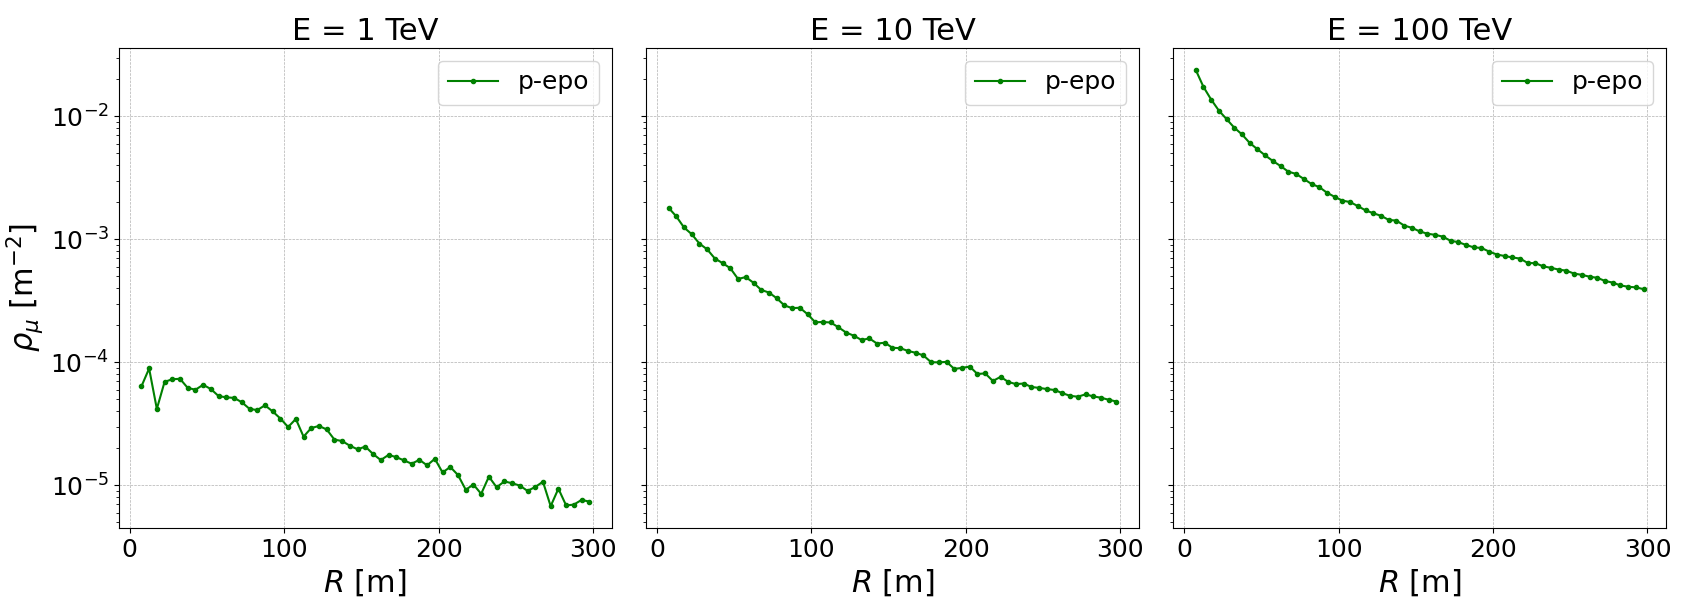
\includegraphics[height=0.4\textheight]{Figuras/lateraldist-pepo}
	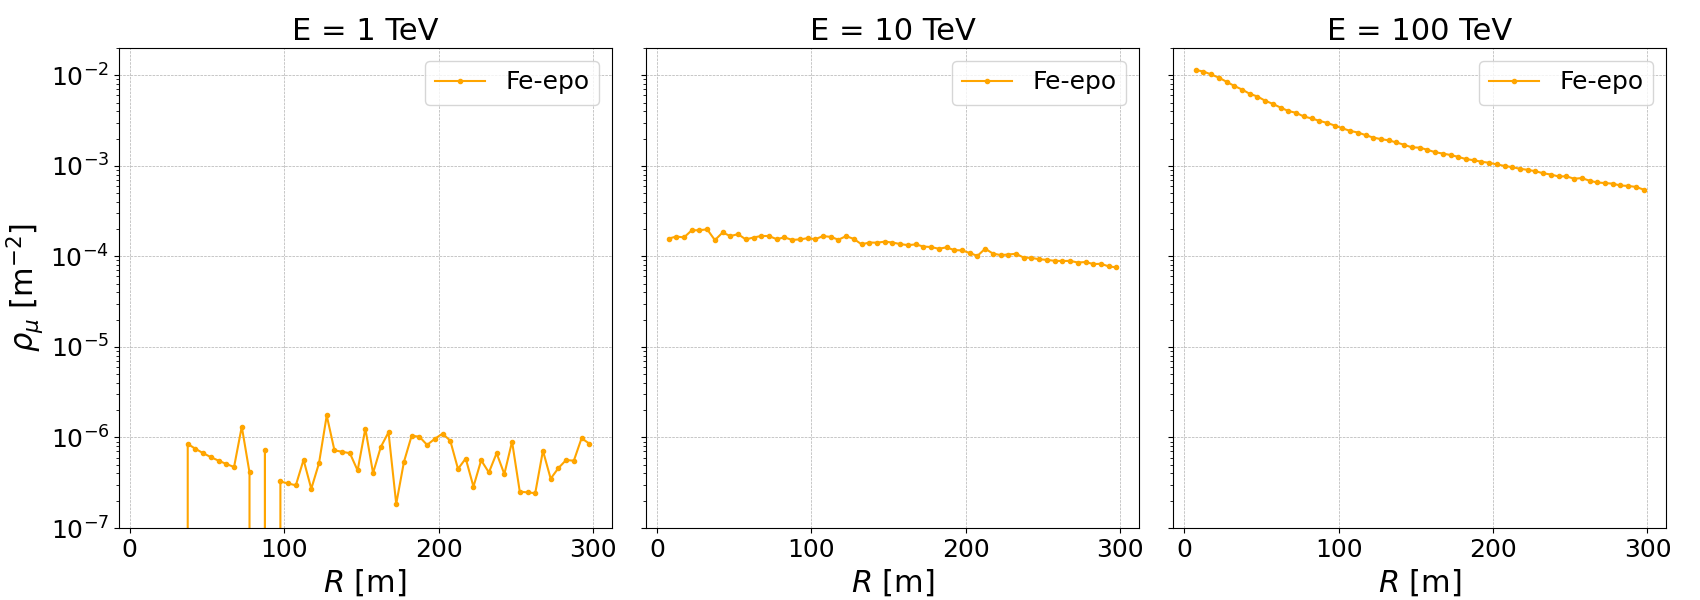
\includegraphics[height=0.4\textheight]{Figuras/lateraldist-Feepo}
	\caption{Resultados preliminares de distribuci\'on lateral de muones con el modelo EPOS-LHC.}
	\end{figure}
\end{frame}


\end{document}